\chapter{Análise Exploratória de Dados}
\label{chap:eda}

\section{Visão Geral}
A análise exploratória foi feita no \textit{script} \texttt{eda\_analysis.py}, que produz um conjunto de gráficos e estatísticas a partir do ficheiro \texttt{cleaned\_data.csv}. O objetivo desta fase foi compreender a distribuição das variáveis, identificar relações diretas entre elas e perceber quais os fatores aparentemente mais ligados ao resultado das dietas. Os gráficos gerados são guardados numa pasta própria e foram usados como base para a análise apresentada neste capítulo.

\section{Análise de Correlações}
O grupo calculou a matriz de correlação de Pearson entre todas as variáveis numéricas e identificou as cinco variáveis mais correlacionadas com a variação de peso aos seis meses, a variável central do problema. A tabela \ref{tab:corr} apresenta esses resultados.

\begin{table}[h]
\centering
\begin{tabular}{|l|c|}
\hline
\textbf{Variável} & \textbf{Correlação com a variação de peso} \\
\hline
\texttt{adherence\_ratio} & $-0,63$ \\
\texttt{mean\_adherence\_pct} & $-0,63$ \\
\texttt{motivation\_score\_program} & $-0,51$ \\
\texttt{baseline\_weight\_kg} & $-0,43$ \\
\texttt{motivation\_score} & $-0,32$ \\
\hline
\end{tabular}
\caption{As cinco variáveis mais correlacionadas com a variação de peso aos seis meses.}
\label{tab:corr}
\end{table}

A leitura destes valores é direta. A adesão ao plano é a variável mais correlacionada com a perda de peso. Como a perda de peso é registada como valor negativo, uma correlação negativa de $-0,63$ significa que quanto maior a adesão, maior a perda. A motivação do paciente segue a mesma lógica. O peso inicial também está associado a maior perda, o que é esperado, já que pacientes mais pesados tendem a perder mais em termos absolutos.

A matriz revelou ainda um facto importante. As variáveis \texttt{adherence\_ratio} e \texttt{mean\_adherence\_pct} apresentam exatamente a mesma correlação com o resultado, o que indica que medem essencialmente a mesma coisa. Esta redundância foi tida em conta na fase de modelação.

A figura \ref{fig:heatmap} apresenta o mapa de calor da matriz de correlação completa, gerado pelo \textit{script}. As zonas mais escuras, vermelhas ou azuis, identificam os pares de variáveis mais correlacionados, e permitem confirmar visualmente as relações descritas.

\begin{figure}[h]
\centering
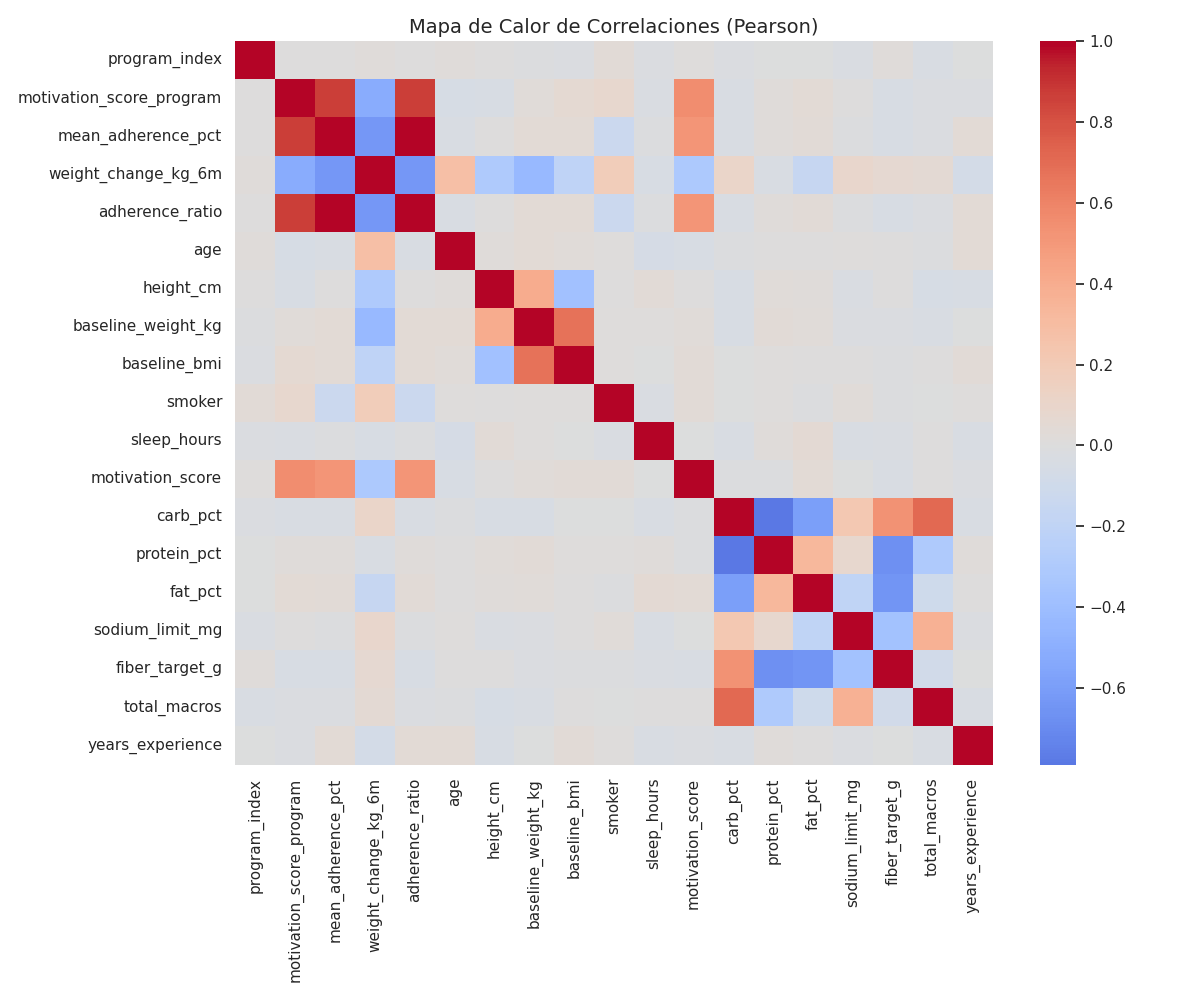
\includegraphics[width=0.9\textwidth]{heatmap_correlacion.png}
\caption{Mapa de calor das correlações de Pearson entre as variáveis numéricas.}
\label{fig:heatmap}
\end{figure}

\section{Resultados por Tipo de Dieta}
A análise da perda média de peso por tipo de dieta mostrou diferenças, embora moderadas. As dietas de baixo teor de hidratos de carbono, agrupadas em \texttt{Low\_carb}, apresentam a maior perda média, próxima de 24 kg. Seguem-se as dietas de base vegetal e as ricas em proteína, e por fim as equilibradas, com perda média de cerca de 21 kg. A diferença entre o melhor e o pior tipo de dieta é de aproximadamente 3 kg em média, o que sugere que o tipo de dieta tem influência, mas não é o fator dominante. A figura \ref{fig:dietas} mostra a distribuição da variação de peso para cada tipo de dieta.

\begin{figure}[h]
\centering
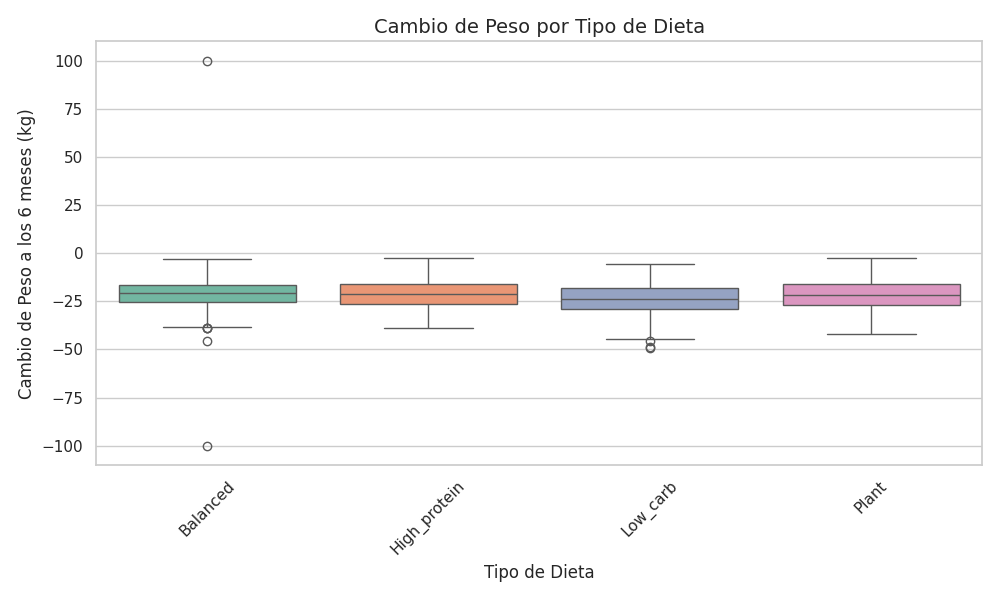
\includegraphics[width=0.8\textwidth]{boxplot_dietas.png}
\caption{Variação de peso aos seis meses por tipo de dieta.}
\label{fig:dietas}
\end{figure}

\section{Resultados por Sexo}
A comparação por sexo revelou uma diferença assinalável. Os pacientes do sexo masculino apresentam uma perda média de cerca de 24,9 kg, enquanto as pacientes do sexo feminino apresentam uma perda média de cerca de 19,3 kg. A diferença média entre os dois grupos é de aproximadamente 5,6 kg.

Esta diferença é relevante, mas deve ser interpretada com cuidado. Parte dela pode dever-se a fatores fisiológicos, já que a perda de peso depende da composição corporal, mas pode também refletir diferenças noutras variáveis distribuídas de forma desigual entre os dois grupos. A figura \ref{fig:sexo} apresenta a distribuição da variação de peso para cada sexo.

\begin{figure}[h]
\centering
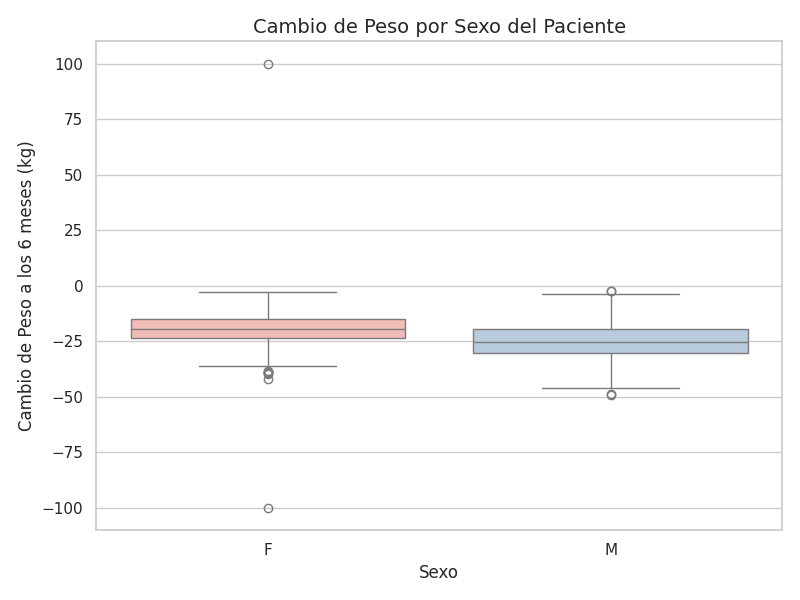
\includegraphics[width=0.65\textwidth]{boxplot_sexo.png}
\caption{Variação de peso aos seis meses por sexo do paciente.}
\label{fig:sexo}
\end{figure}

Importa ainda referir que foi precisamente esta análise por sexo que tornou visível o problema de inconsistência na coluna \texttt{sex}, descrito no capítulo anterior. Numa execução inicial, o resumo apresentou oito grupos em vez de dois, o que levou o grupo a reforçar a normalização desta coluna.

\section{Influência do Perfil do Nutricionista}
O grupo analisou o efeito da abordagem do nutricionista no resultado das dietas. Os resultados mostram que a abordagem mais exigente, identificada como \texttt{Strict}, está associada à maior perda média de peso, cerca de 23,8 kg. As abordagens \texttt{Motivational} e \texttt{Empathetic} situam-se em valores intermédios, e a abordagem \texttt{Data\_driven} apresenta a menor perda média, cerca de 20,4 kg. Já a especialidade do nutricionista mostrou pouca influência, com perdas médias muito próximas entre as quatro especialidades, todas entre 21,7 e 22,1 kg. A figura \ref{fig:nutricionista} apresenta a perda média de peso para cada abordagem.

\begin{figure}[h]
\centering
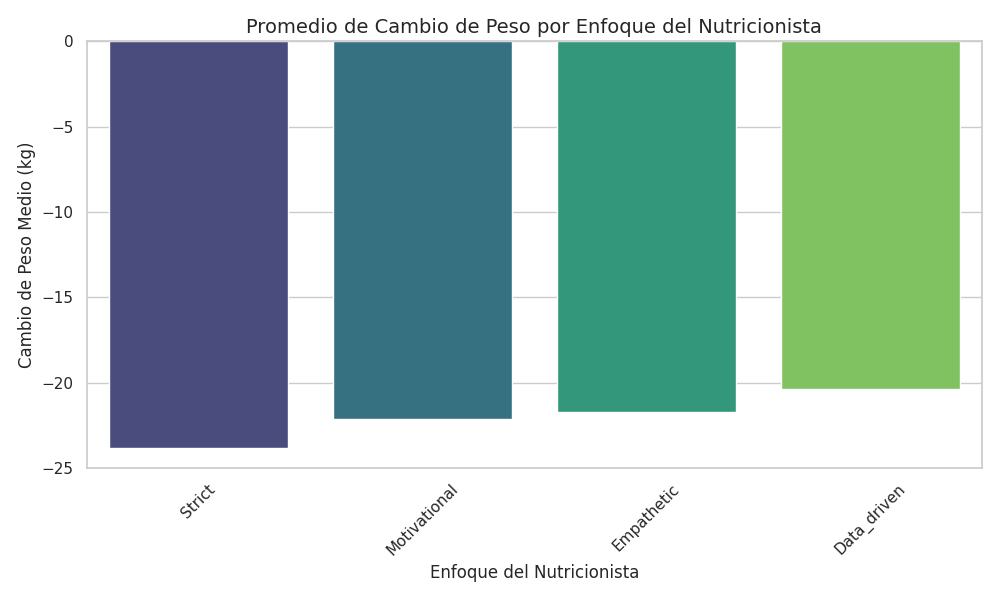
\includegraphics[width=0.8\textwidth]{barras_nutricionista.png}
\caption{Perda média de peso por abordagem do nutricionista.}
\label{fig:nutricionista}
\end{figure}

\section{Síntese da Análise}
Desta fase ficaram duas conclusões principais. A primeira é que o comportamento do paciente, traduzido na adesão e na motivação, é de longe o fator mais ligado ao resultado, mais do que qualquer característica da dieta ou do nutricionista. A segunda é que existem variáveis redundantes no conjunto, nomeadamente o par formado pela adesão e pelo rácio de adesão, que devem ser tratadas com cuidado na modelação.
